\documentclass[12pt,parskip=full]{scrartcl}
\usepackage[utf8]{inputenc}   % UTF8-Kodierung für Umlaute
\usepackage{ngerman}          % deutsche Silbentrennung
\usepackage[T1]{fontenc}	  % wichtig für Trennung von Wörtern mit Umlauten
\usepackage{microtype}		  % verbesserter Randausgleich
\usepackage{graphicx}         % Einbindung von Grafiken
\usepackage{wrapfig}			% Grafiken im Text
\usepackage{subcaption}         % Für Subgrafiken

\title{Ausführliche Nähanleitung Mund-Nasen-Schutz mit Nackenband}
\author{Anna Klingauf}
\date{Oktober 2020}

\begin{document}
\begin{titlepage}
\maketitle
\thispagestyle{empty}
\begin{figure}[b!] 
  \centering
     
\includegraphics[width=0.60\textwidth]{Pictures/00_Completed/Gesamt.png}
\end{figure}
\end{titlepage}
\clearpage

\section{Allgemeines}
Der Mund-Nasen-Schutz (abgekürzt MNS oder Maske) wie er hier vorgestellt wird besteht aus zwei Lagen Baumwollstoff. Im Gegensatz zu den meisten anderen MNS wird er nicht an den Ohren befestigt sondern mit einem elastischen Band im Nacken. Das Band kann mit Klett, Knöpfen oder Druckknöpfen geschlossen werden. An der Nase ist sowohl ein Drahteinsatz als auch eine Abdichtung mit Gummi angebracht. Da die Maske durch die Form und die Abdichtung an der Nase sehr dicht ist, beschlägt bei allen bisherigen Testpersonen die Brille nicht. Die Faltung der Maske kann beim Nähen individuell an das Gesicht angepasst werden. Es werden drei Größen als Vorschläge zur Verfügung gestellt, die auch individuell angepasst werden können.

\section{Materialien}
Folgende Materialien werden benötigt:
\begin{itemize}
    \item Außenstoff (2 mal ca. 17 x 19 cm), z.B Baumwolle
    \item Innenstoff (2 mal ca. 17 x 19 cm), z.B. Baumwolle
    \item Rest-Stoff (für Drahteinsatz, ca 4 x 10 cm)
    \item 2 Büroklammern, am besten mit Plastiküberzug
    \item Abdichtung, ca. 7 cm, z.B. aus halterlosen Strümpfen
    \item elastisches Band, ca. 45 cm lang, je nach Größe
    \item Verschluss: Klettband oder Knöpfe oder Druckknöpfe
\end{itemize}

Folgende Werkzeuge werden benötigt:
\begin{itemize}
    \item Nähmaschine
    \item Schere
    \item Stecknadeln
    \item Sicherheitsnadel
    \item Schnittmuster (ausgeschnitten)
    \item ggf. Nadel und Faden (zum Annähen der Knöpfe oder Druckknöpfe)
    \item ggf. Stift oder Stab (als Hilfe zum Drehen der Maske)
    \item ggf. Bügeleisen (um den Stoff vorher vorzubereiten falls nötig)
\end{itemize}

\begin{figure}[h]
    \vspace{0.5cm}
    \centering
    \begin{subfigure}{0.48\textwidth}
        \centering
        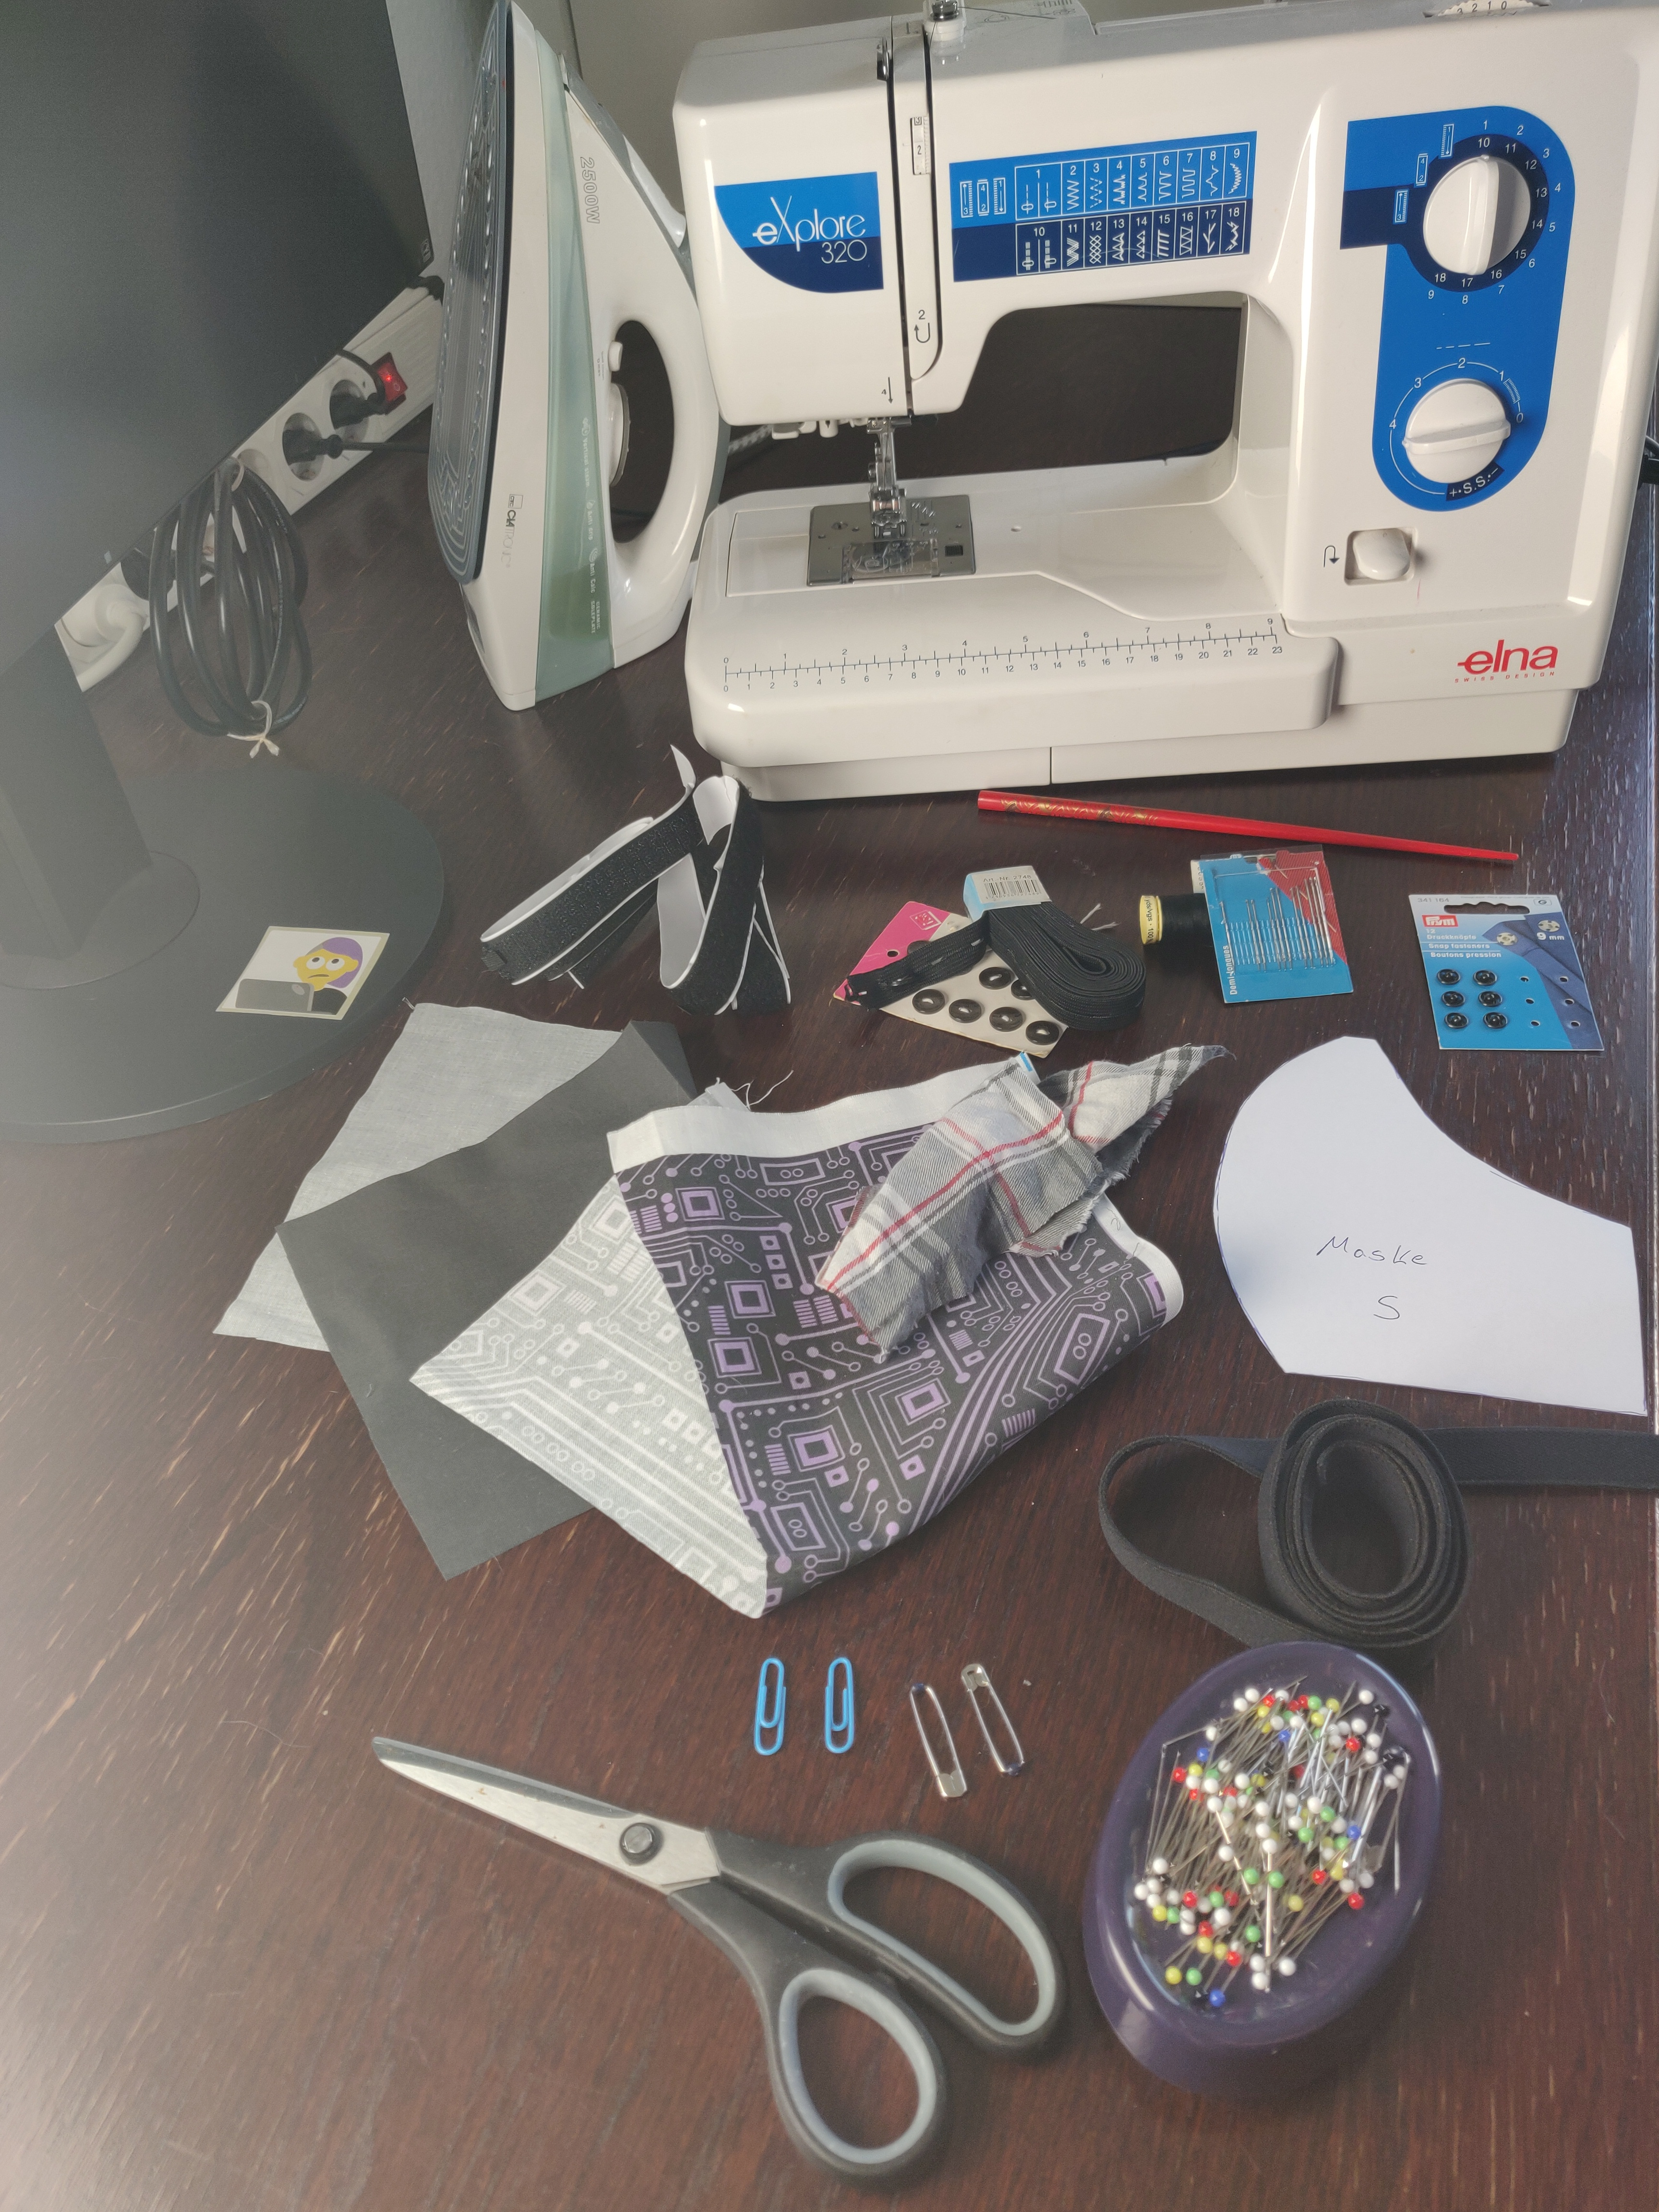
\includegraphics[width = \linewidth]{Pictures/01_Materials/materials_01.jpg}
        \caption{Übericht}
    \end{subfigure}
    \begin{subfigure}{0.48\textwidth}
        \centering
        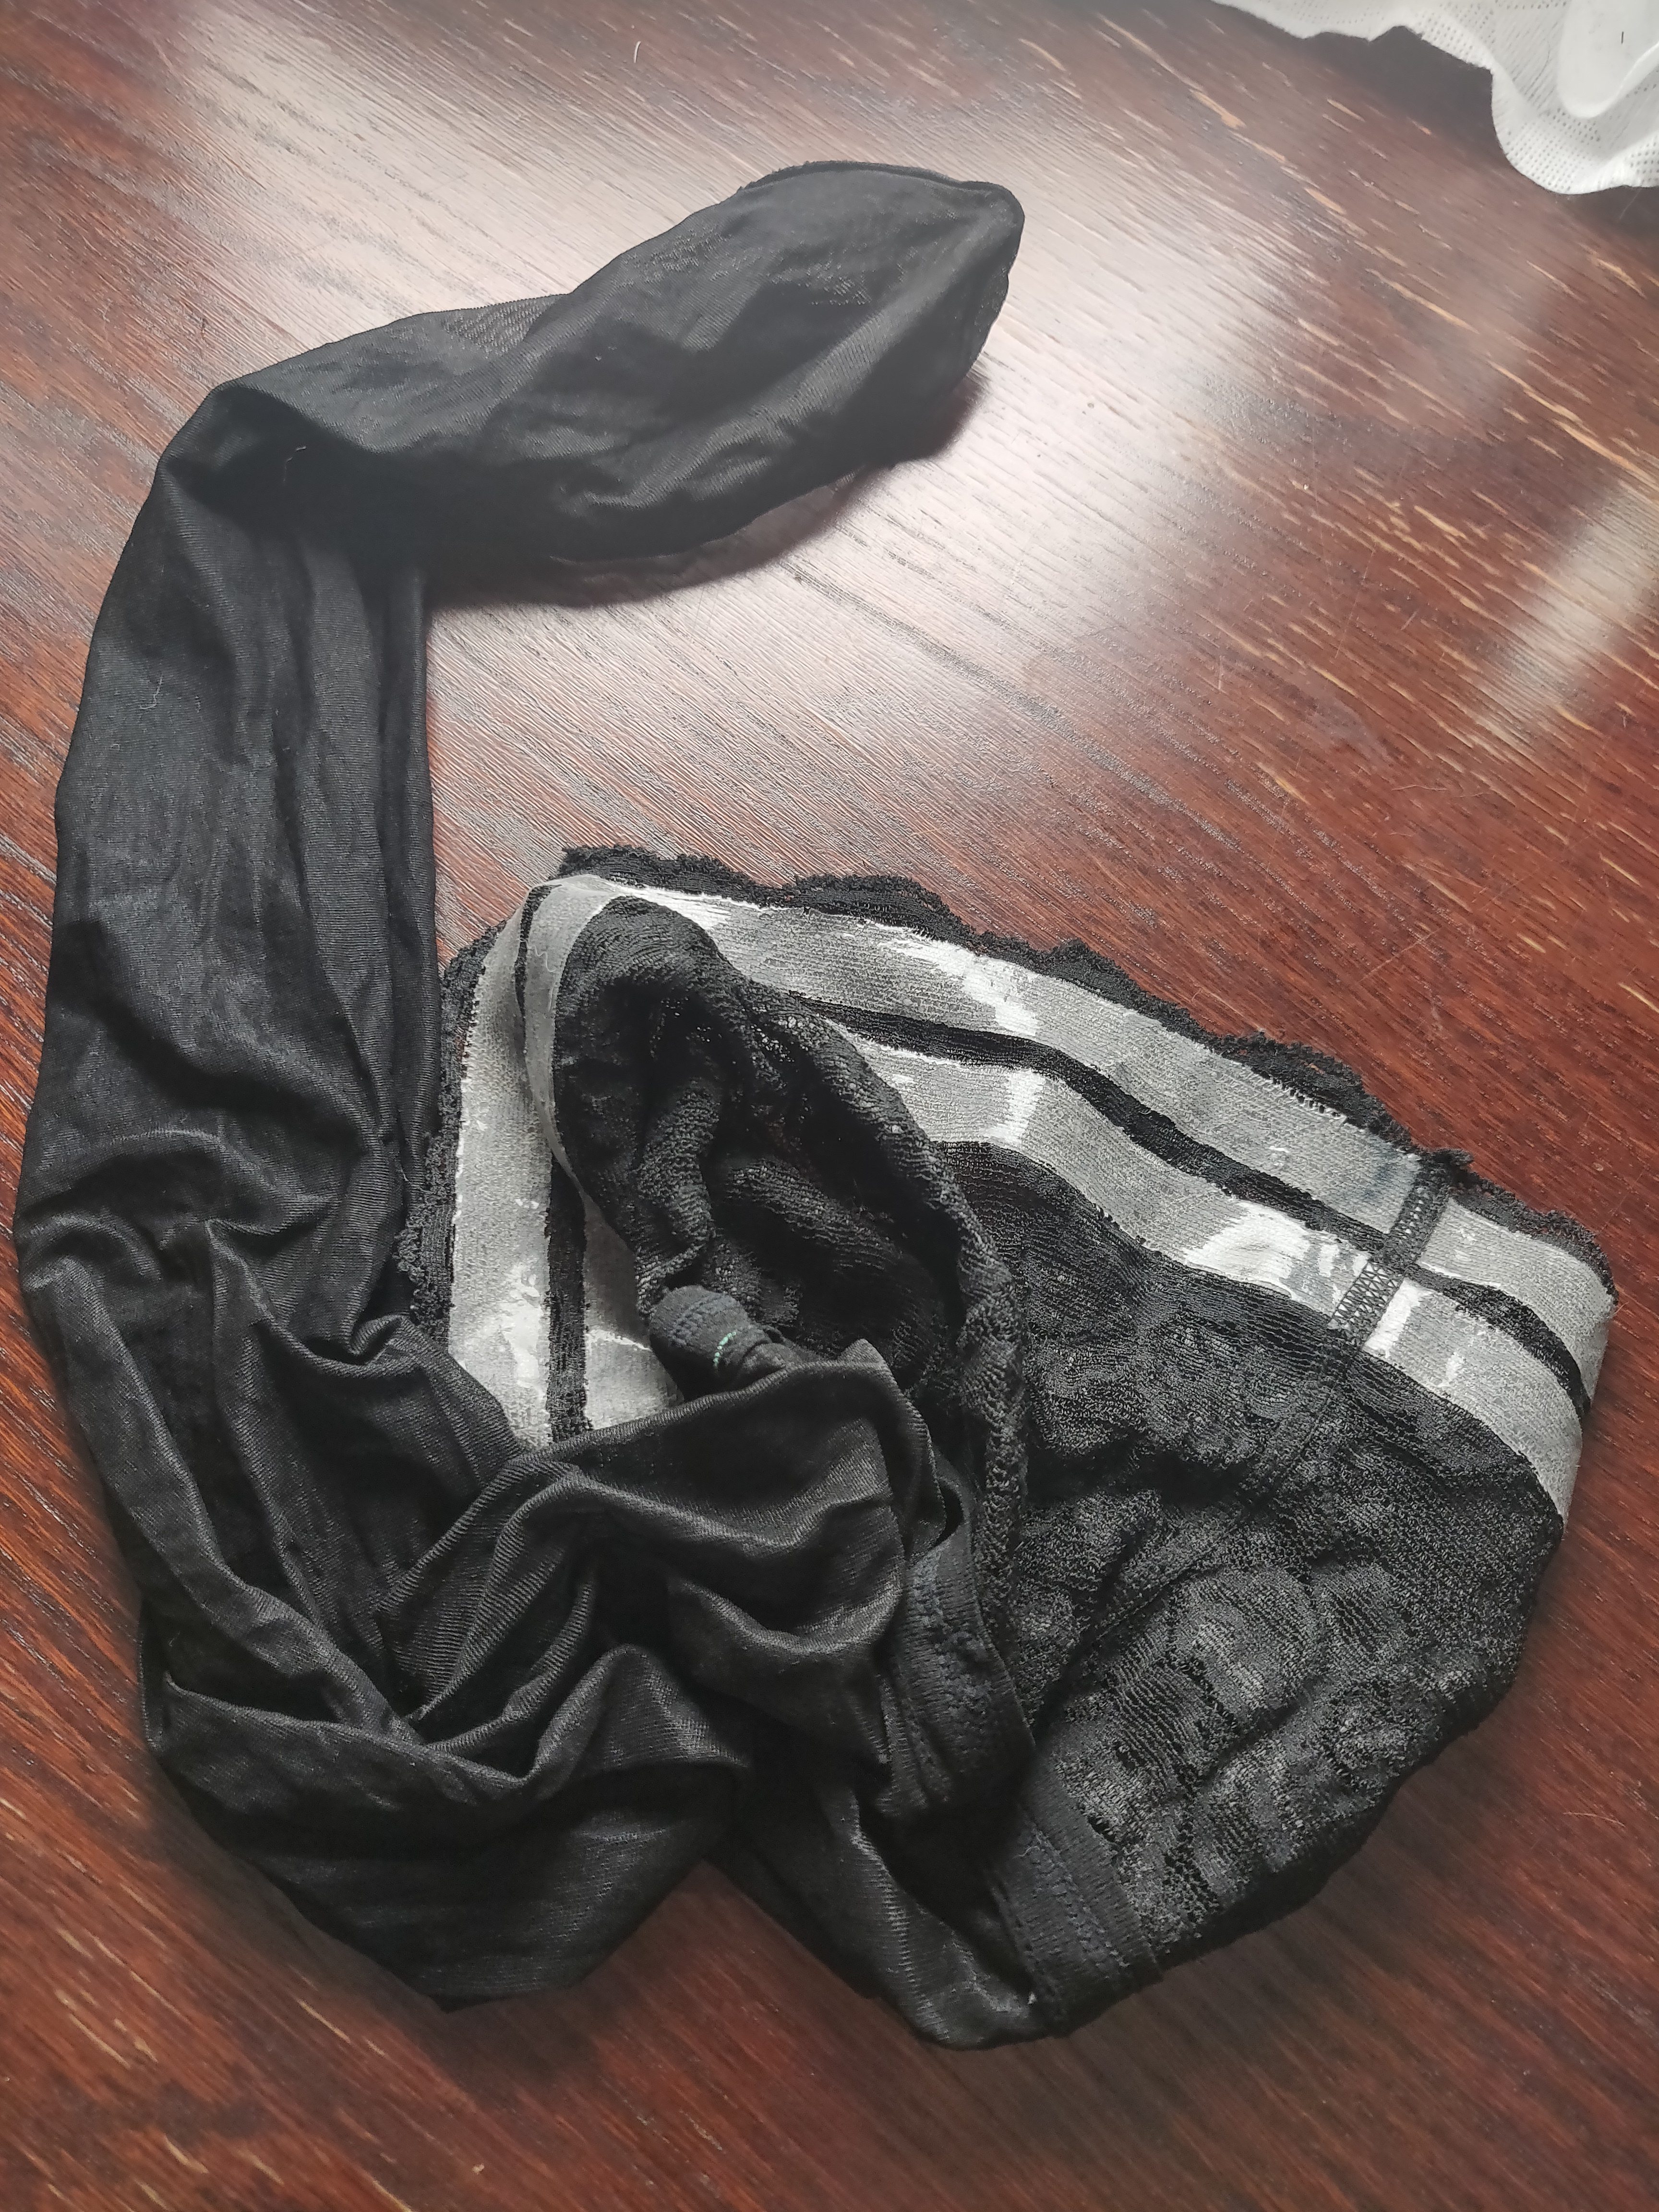
\includegraphics[width = \linewidth]{Pictures/01_Materials/materials_02.jpg}
        \caption{Abdichtung aus halterlosen Strümpfen}
    \end{subfigure}
    \caption{Materialien und Werkzeuge}
\end{figure}

\section{Drahteinsatz}
Als Drahteinsatz kommen hier zwei beschichtete Büroklammern zum Einsatz. Die Beschichtung ist hilfreich, da das Metall so gut vor Wasser geschützt ist und weniger schnell rostet. Alternativ zu Böroklammern können auch andere Metallstücke verwendet werden, die leicht zu biegen und nicht zu scharfkantig sind. Die Büroklammern werden in Stoff eingenäht, um sie einerseits fest in der Maske zu vernähen (damit sie nicht rutschen) und andererseits um zu verhindern, dass die Klammern durch den Stoff der Maske stechen. Dieser Schritt kann auch später durchgeführt werden, es ergibt aber Sinn, sich bei diesem Teil (wieder) mit dem feststecken und Nähen vertraut zu machen, da man dieses Stück nicht sieht.\par

Die Büroklammern werden zuerst gerade gebogen und etwas gekürzt, so dass sie etwa 7 cm lang sind (siehe Abbildung \ref{MetaStrip1}). Dann wird aus dem Rest-Stoff ein Stück ausgeschnitten, das groß genug ist, um die Drahtstücke locker darin einzuschlagen und festzustecken (siehe Abbildung \ref{MetaStrip2}). Die Seiten des Stoffs werden nach innen eingeschlagen und ebenfalls mit Nadeln festgesteckt (siehe Abbildung \ref{MetaStrip3}). Dabei sollten die Nadeln so positioniert werden, dass sie im rechten Winkel zu den Büroklammern und somit auch im rechten Winkel zu der geplanten Naht stecken, ohne dass das Füßchen der Nähmaschine an den Stecknadelköpfen hängen bleibt. Die richtige Positionierung der Stecknadeln kann man an diesem Stück gut für die anderen Nähte ausprobieren. Anschließend wird die Naht parallel zu den Büroklammern gesetzt, so dass die Klammern gut im Stoffstück eingenäht sind. Überflüssiger Stoff auf der anderen Seite der Naht kann einfach abgeschnitten werden, jedoch nicht zu eng. Das Endergebnis sollte Abbildung \ref{MetaStrip4} ähneln.

\begin{figure}[h]
    \vspace{0.5cm}
    \centering
    \begin{subfigure}{0.48\textwidth}
        \centering
        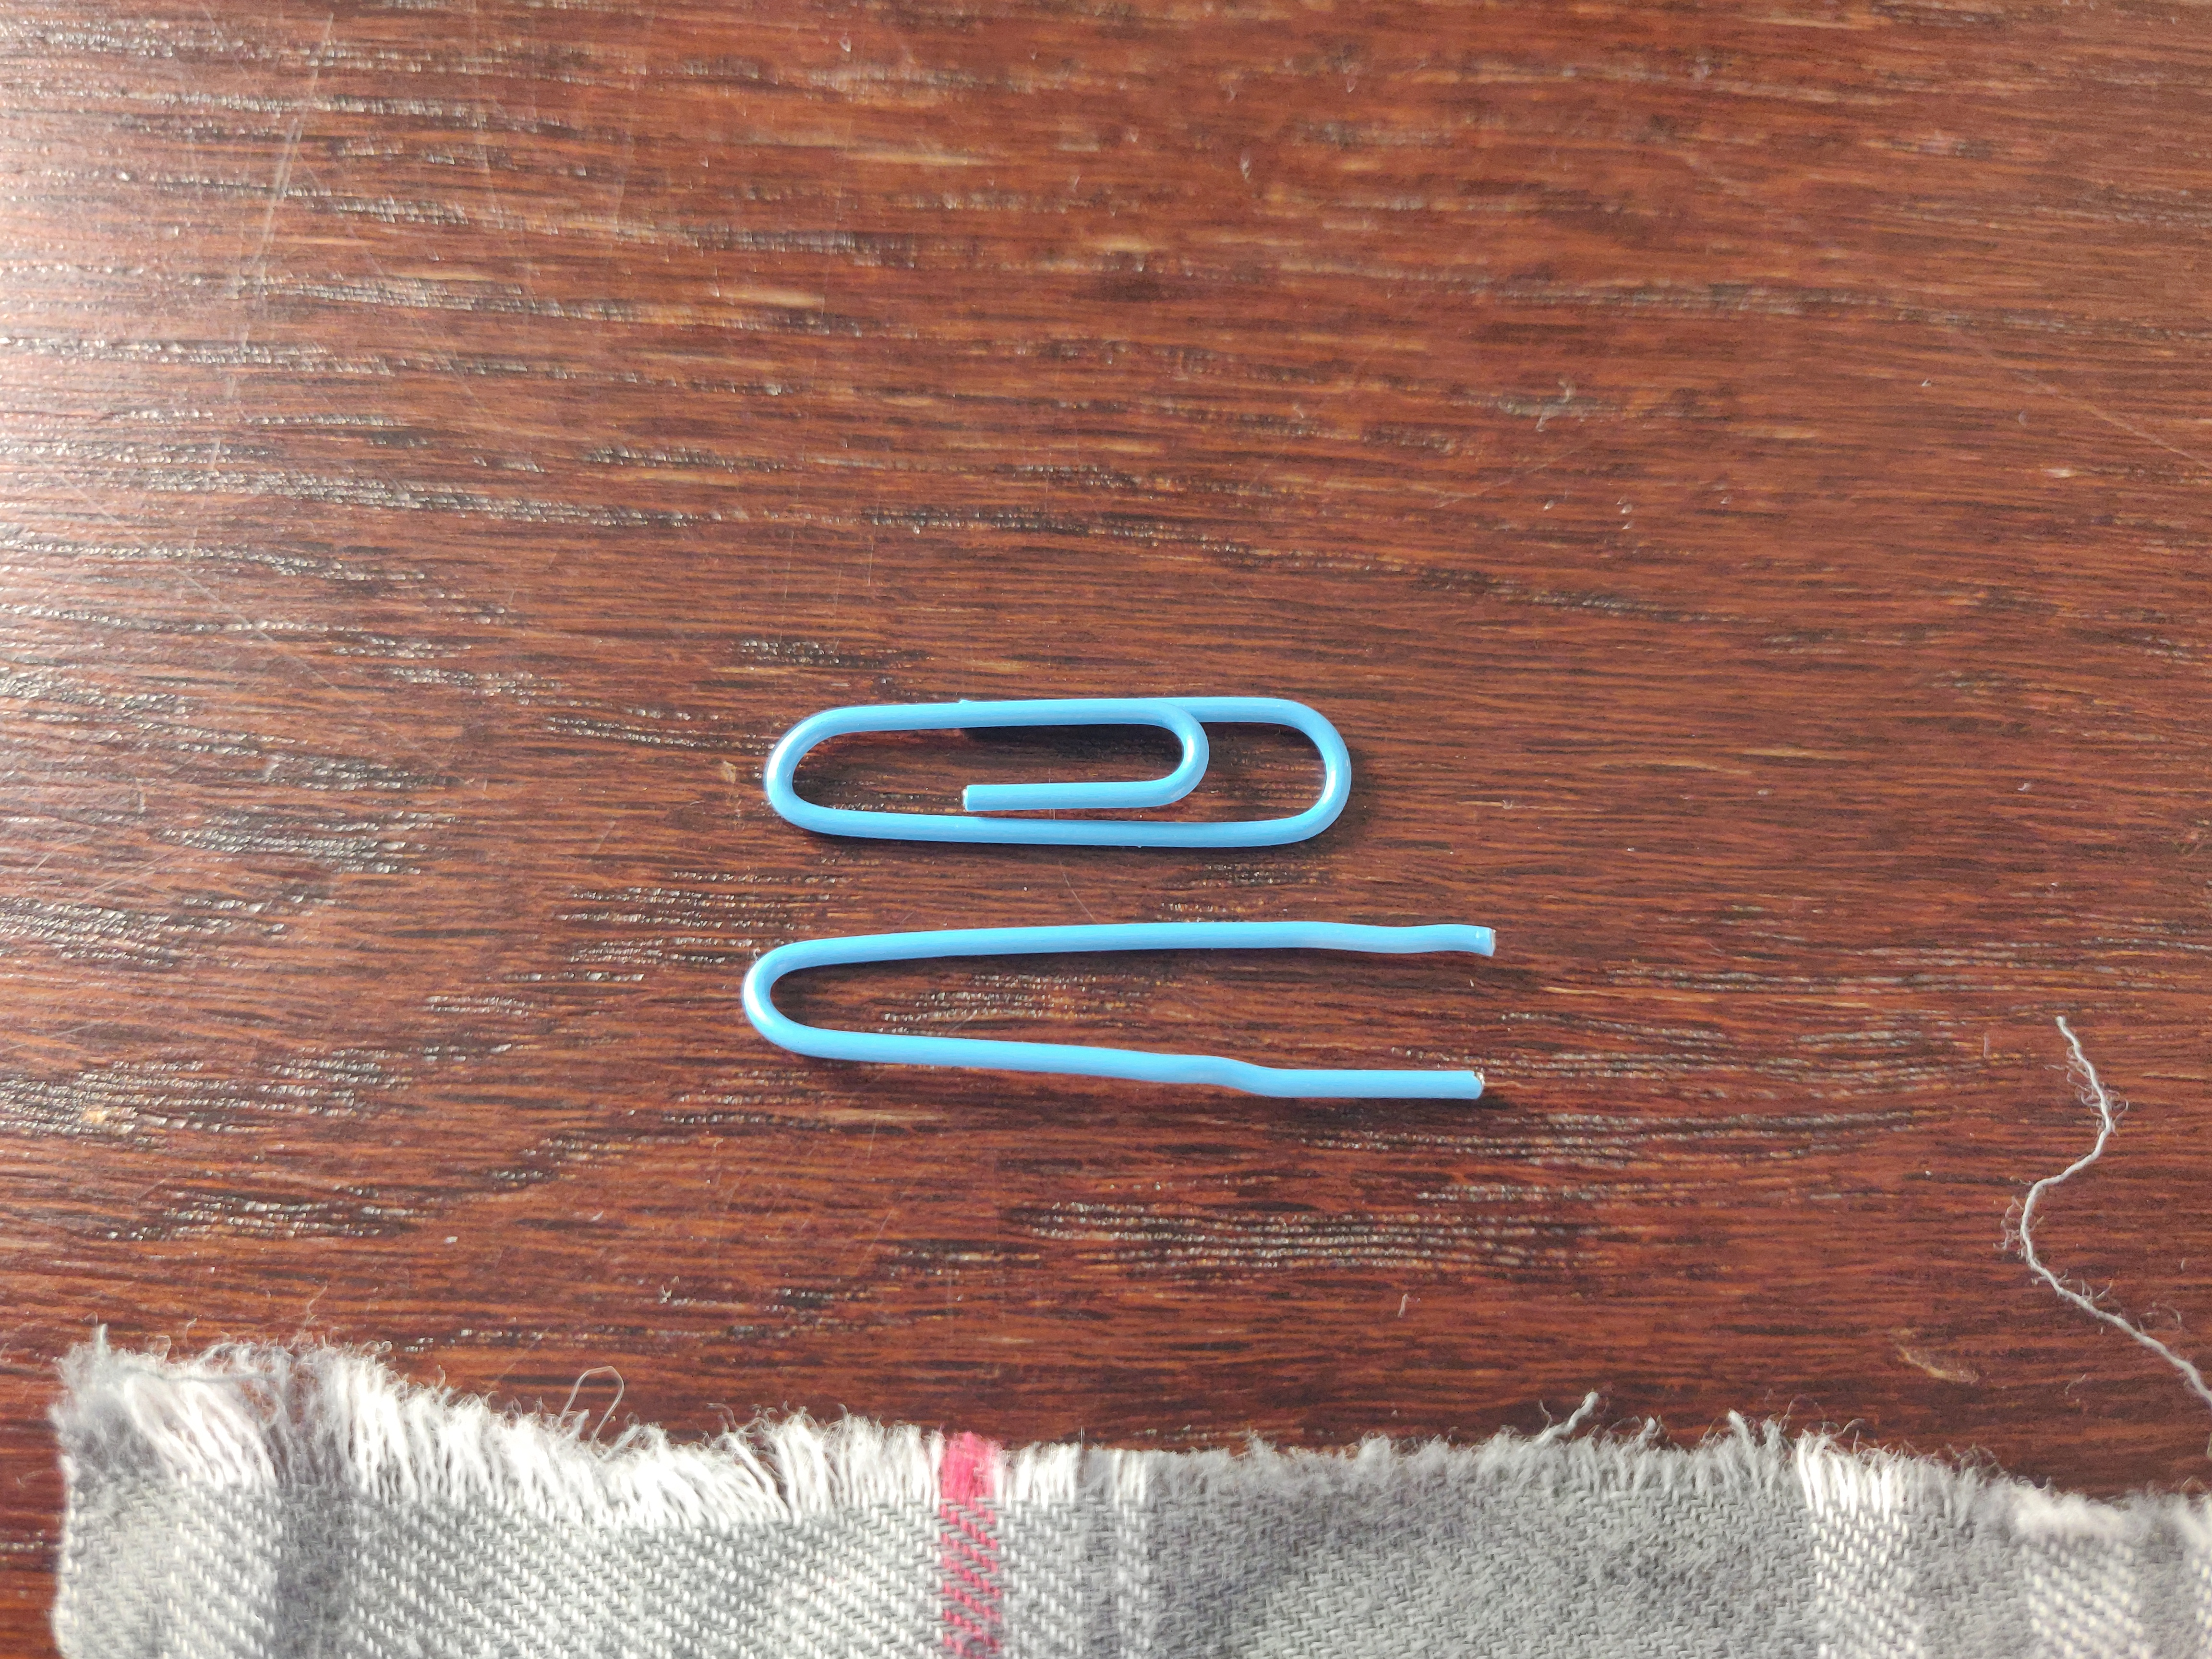
\includegraphics[width = \linewidth]{Pictures/02_MetalStrip/MetalStrip_01.jpg}
        \caption{Biegen und zuschneiden}
        \label{MetaStrip1}
    \end{subfigure}
    \begin{subfigure}{0.48\textwidth}
        \centering
        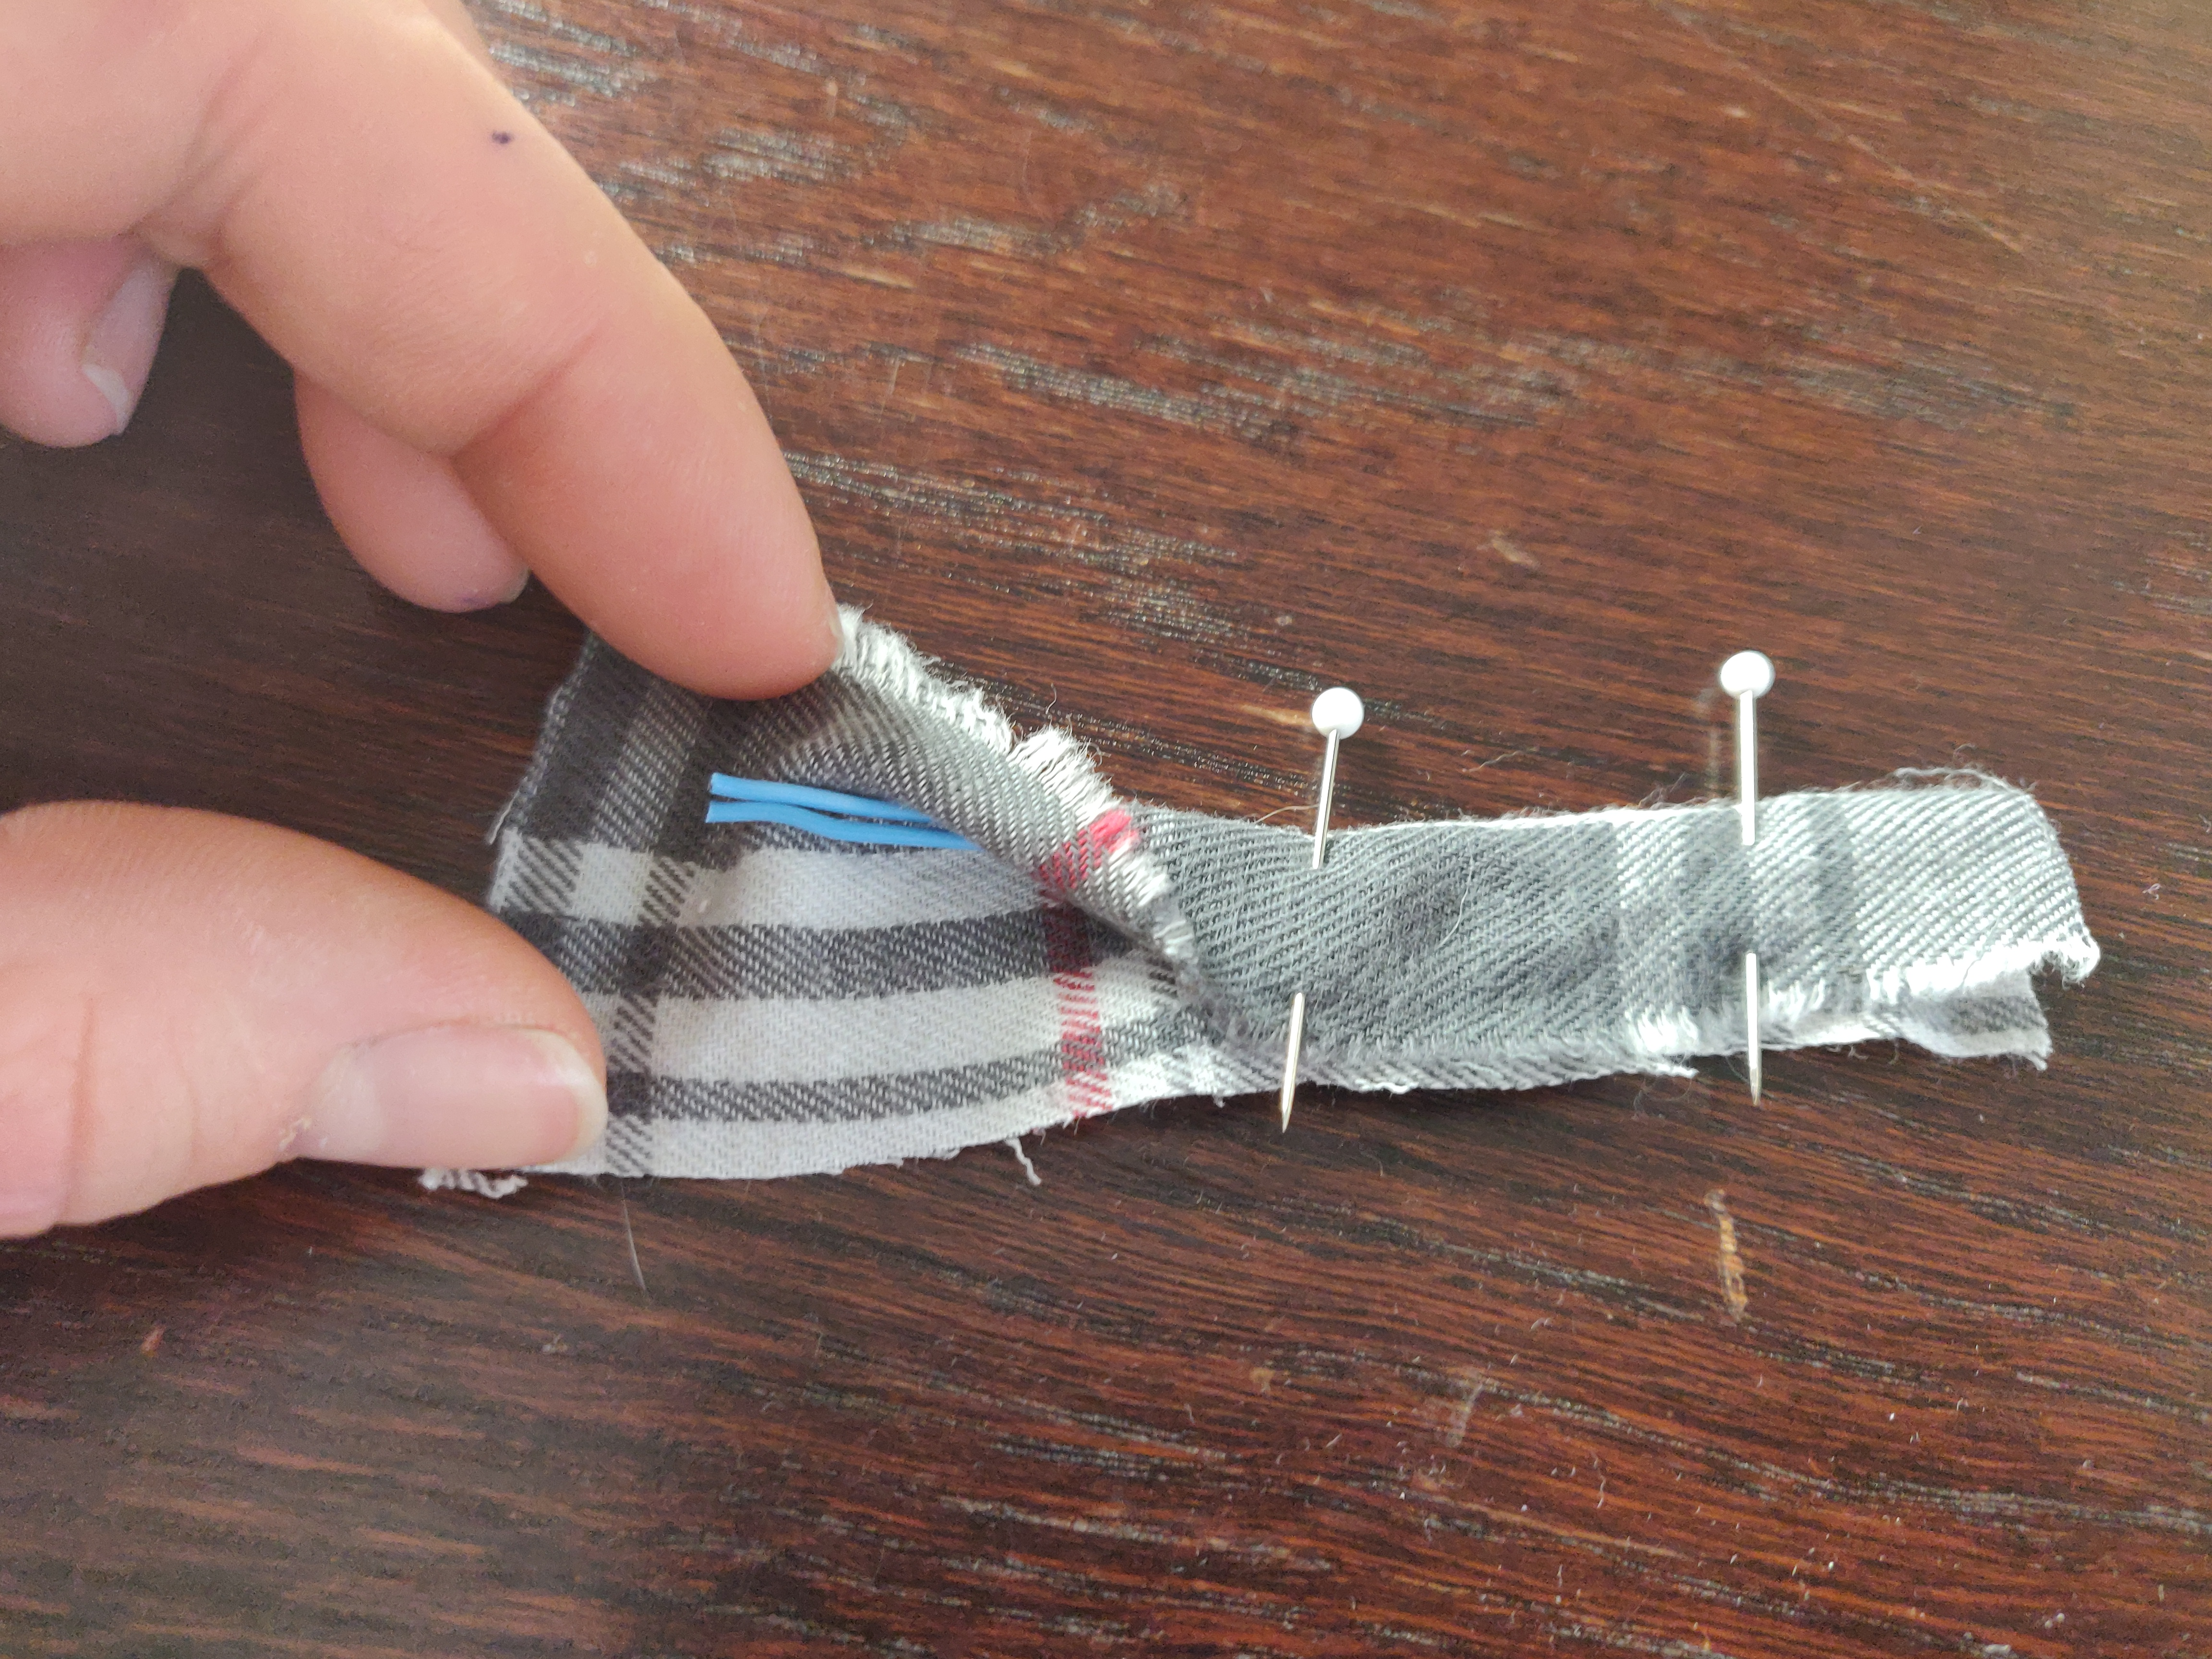
\includegraphics[width = \linewidth]{Pictures/02_MetalStrip/MetalStrip_02.jpg}
        \caption{Einschlagen}
        \label{MetaStrip2}
    \end{subfigure}
    \begin{subfigure}{0.48\textwidth}
        \centering
        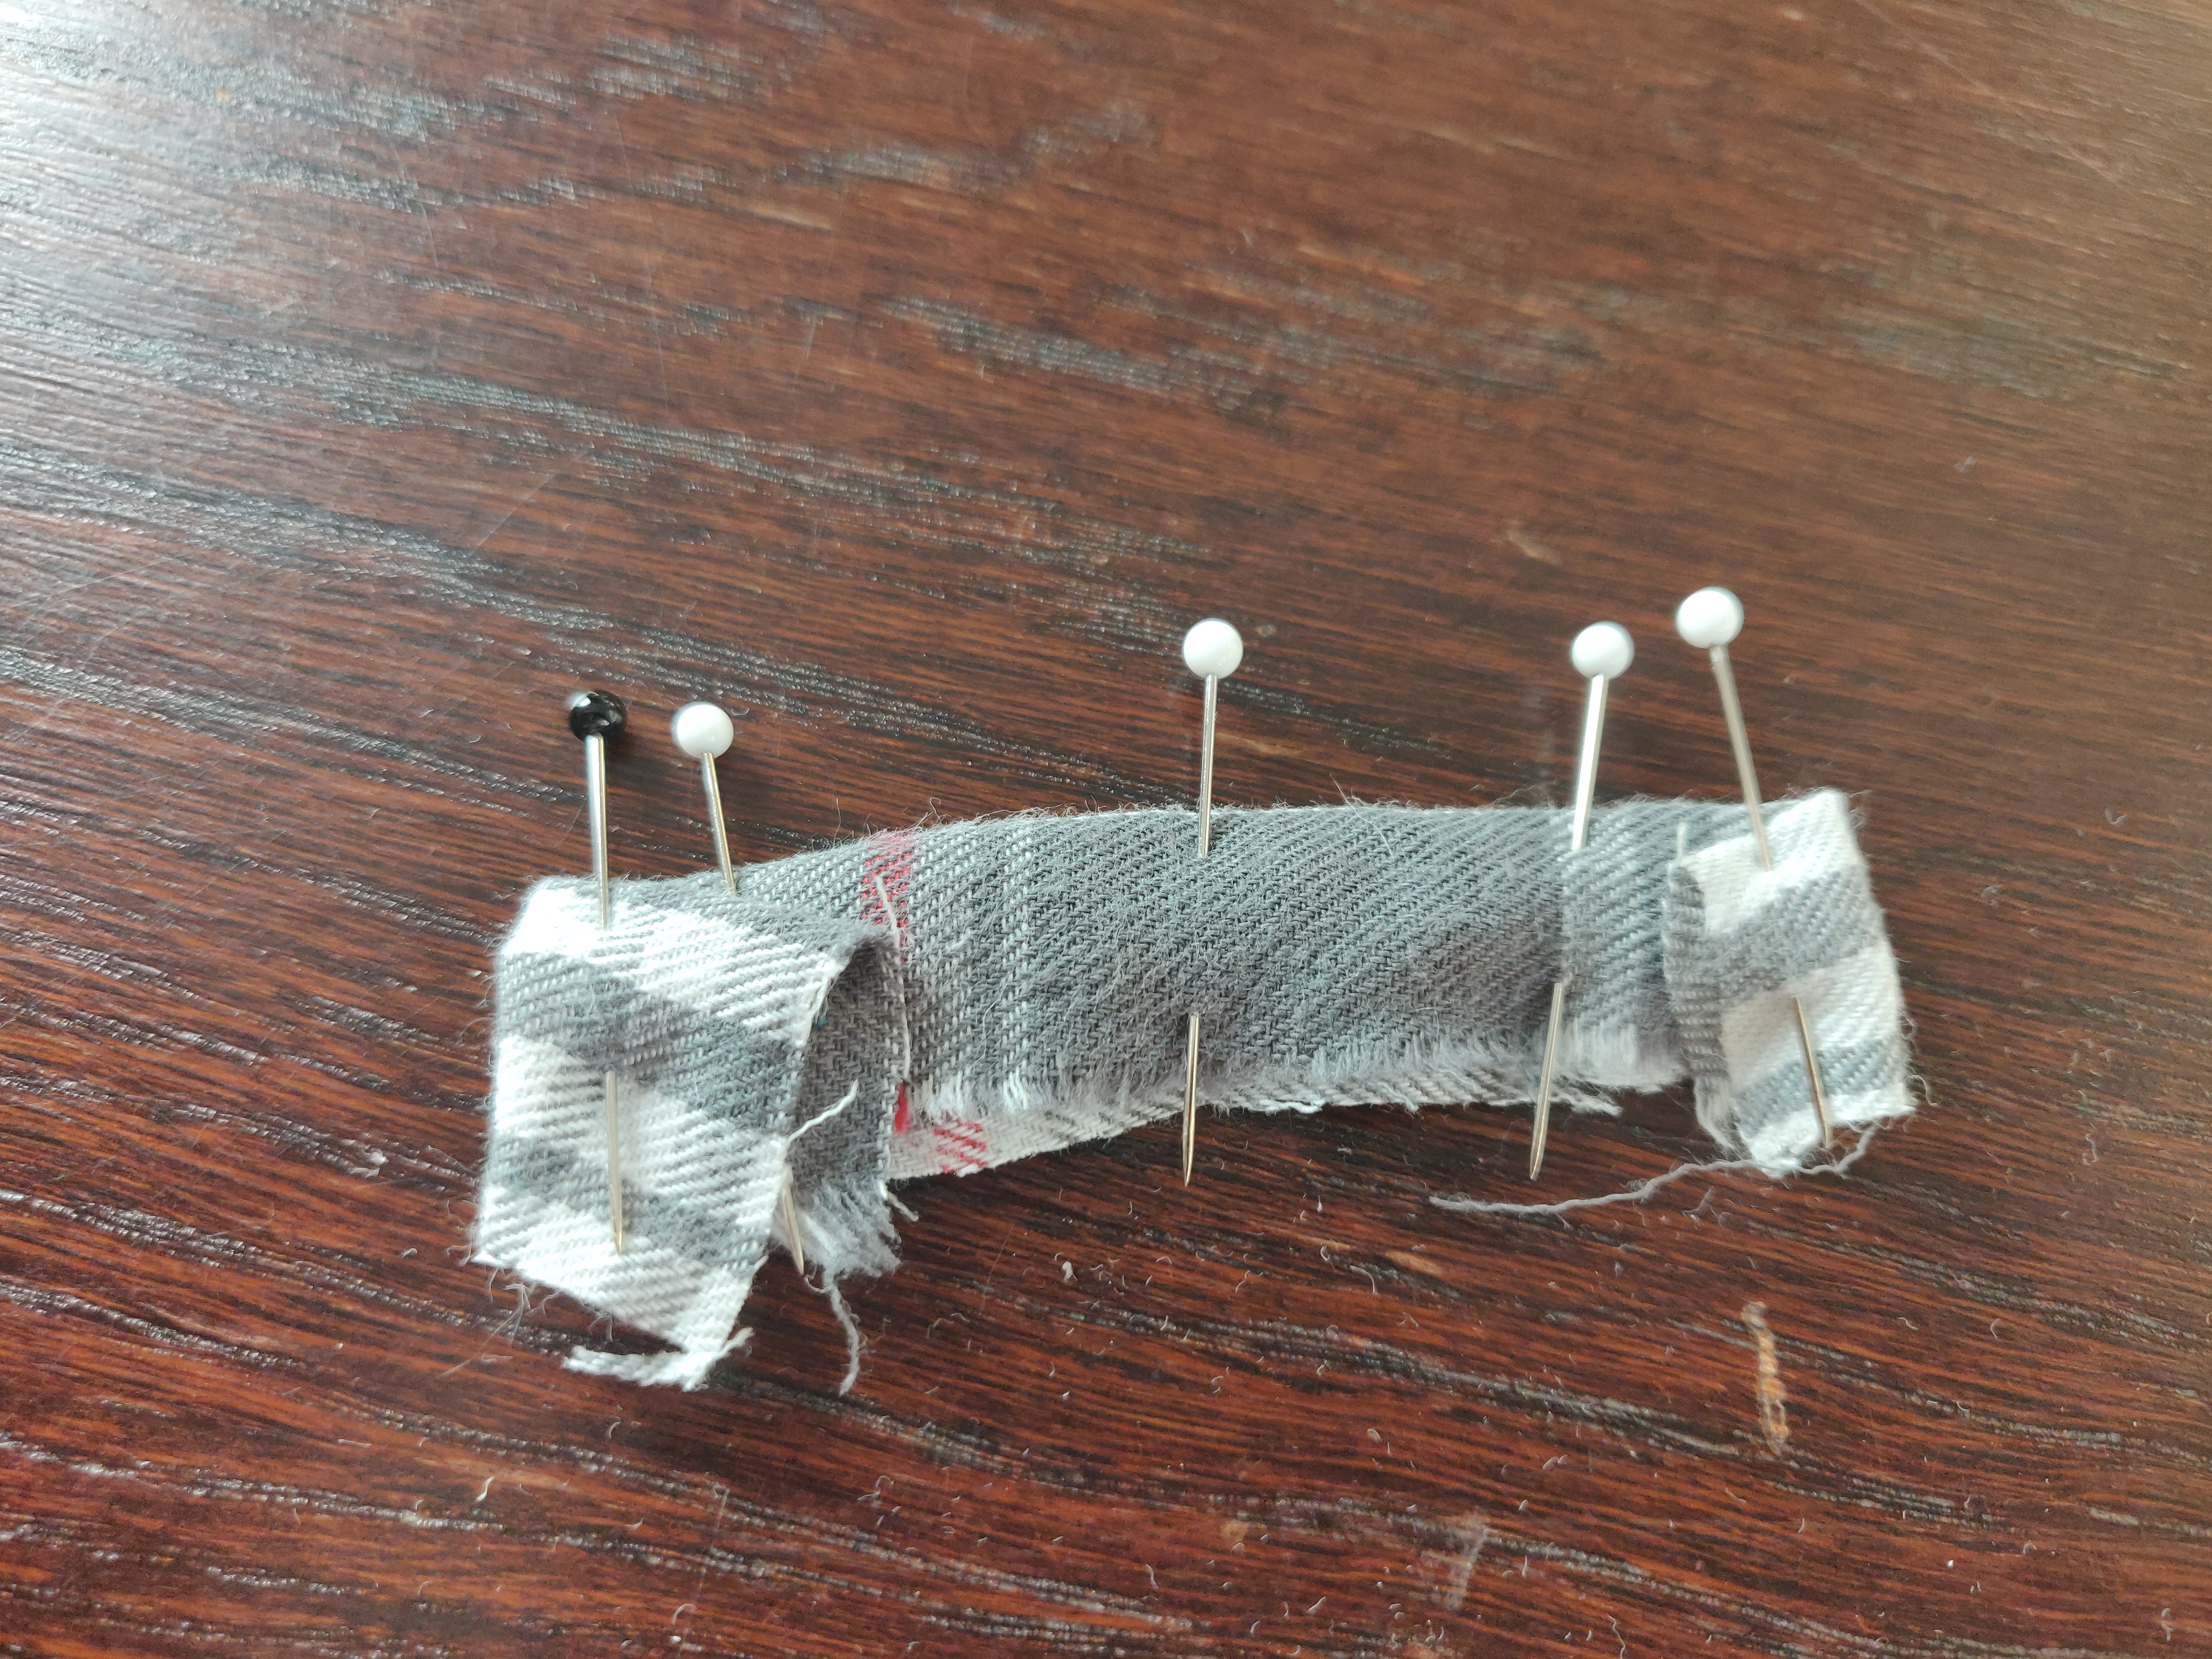
\includegraphics[width = \linewidth]{Pictures/02_MetalStrip/MetalStrip_03.jpg}
        \caption{Feststecken}
        \label{MetaStrip3}
    \end{subfigure}
    \begin{subfigure}{0.48\textwidth}
        \centering
        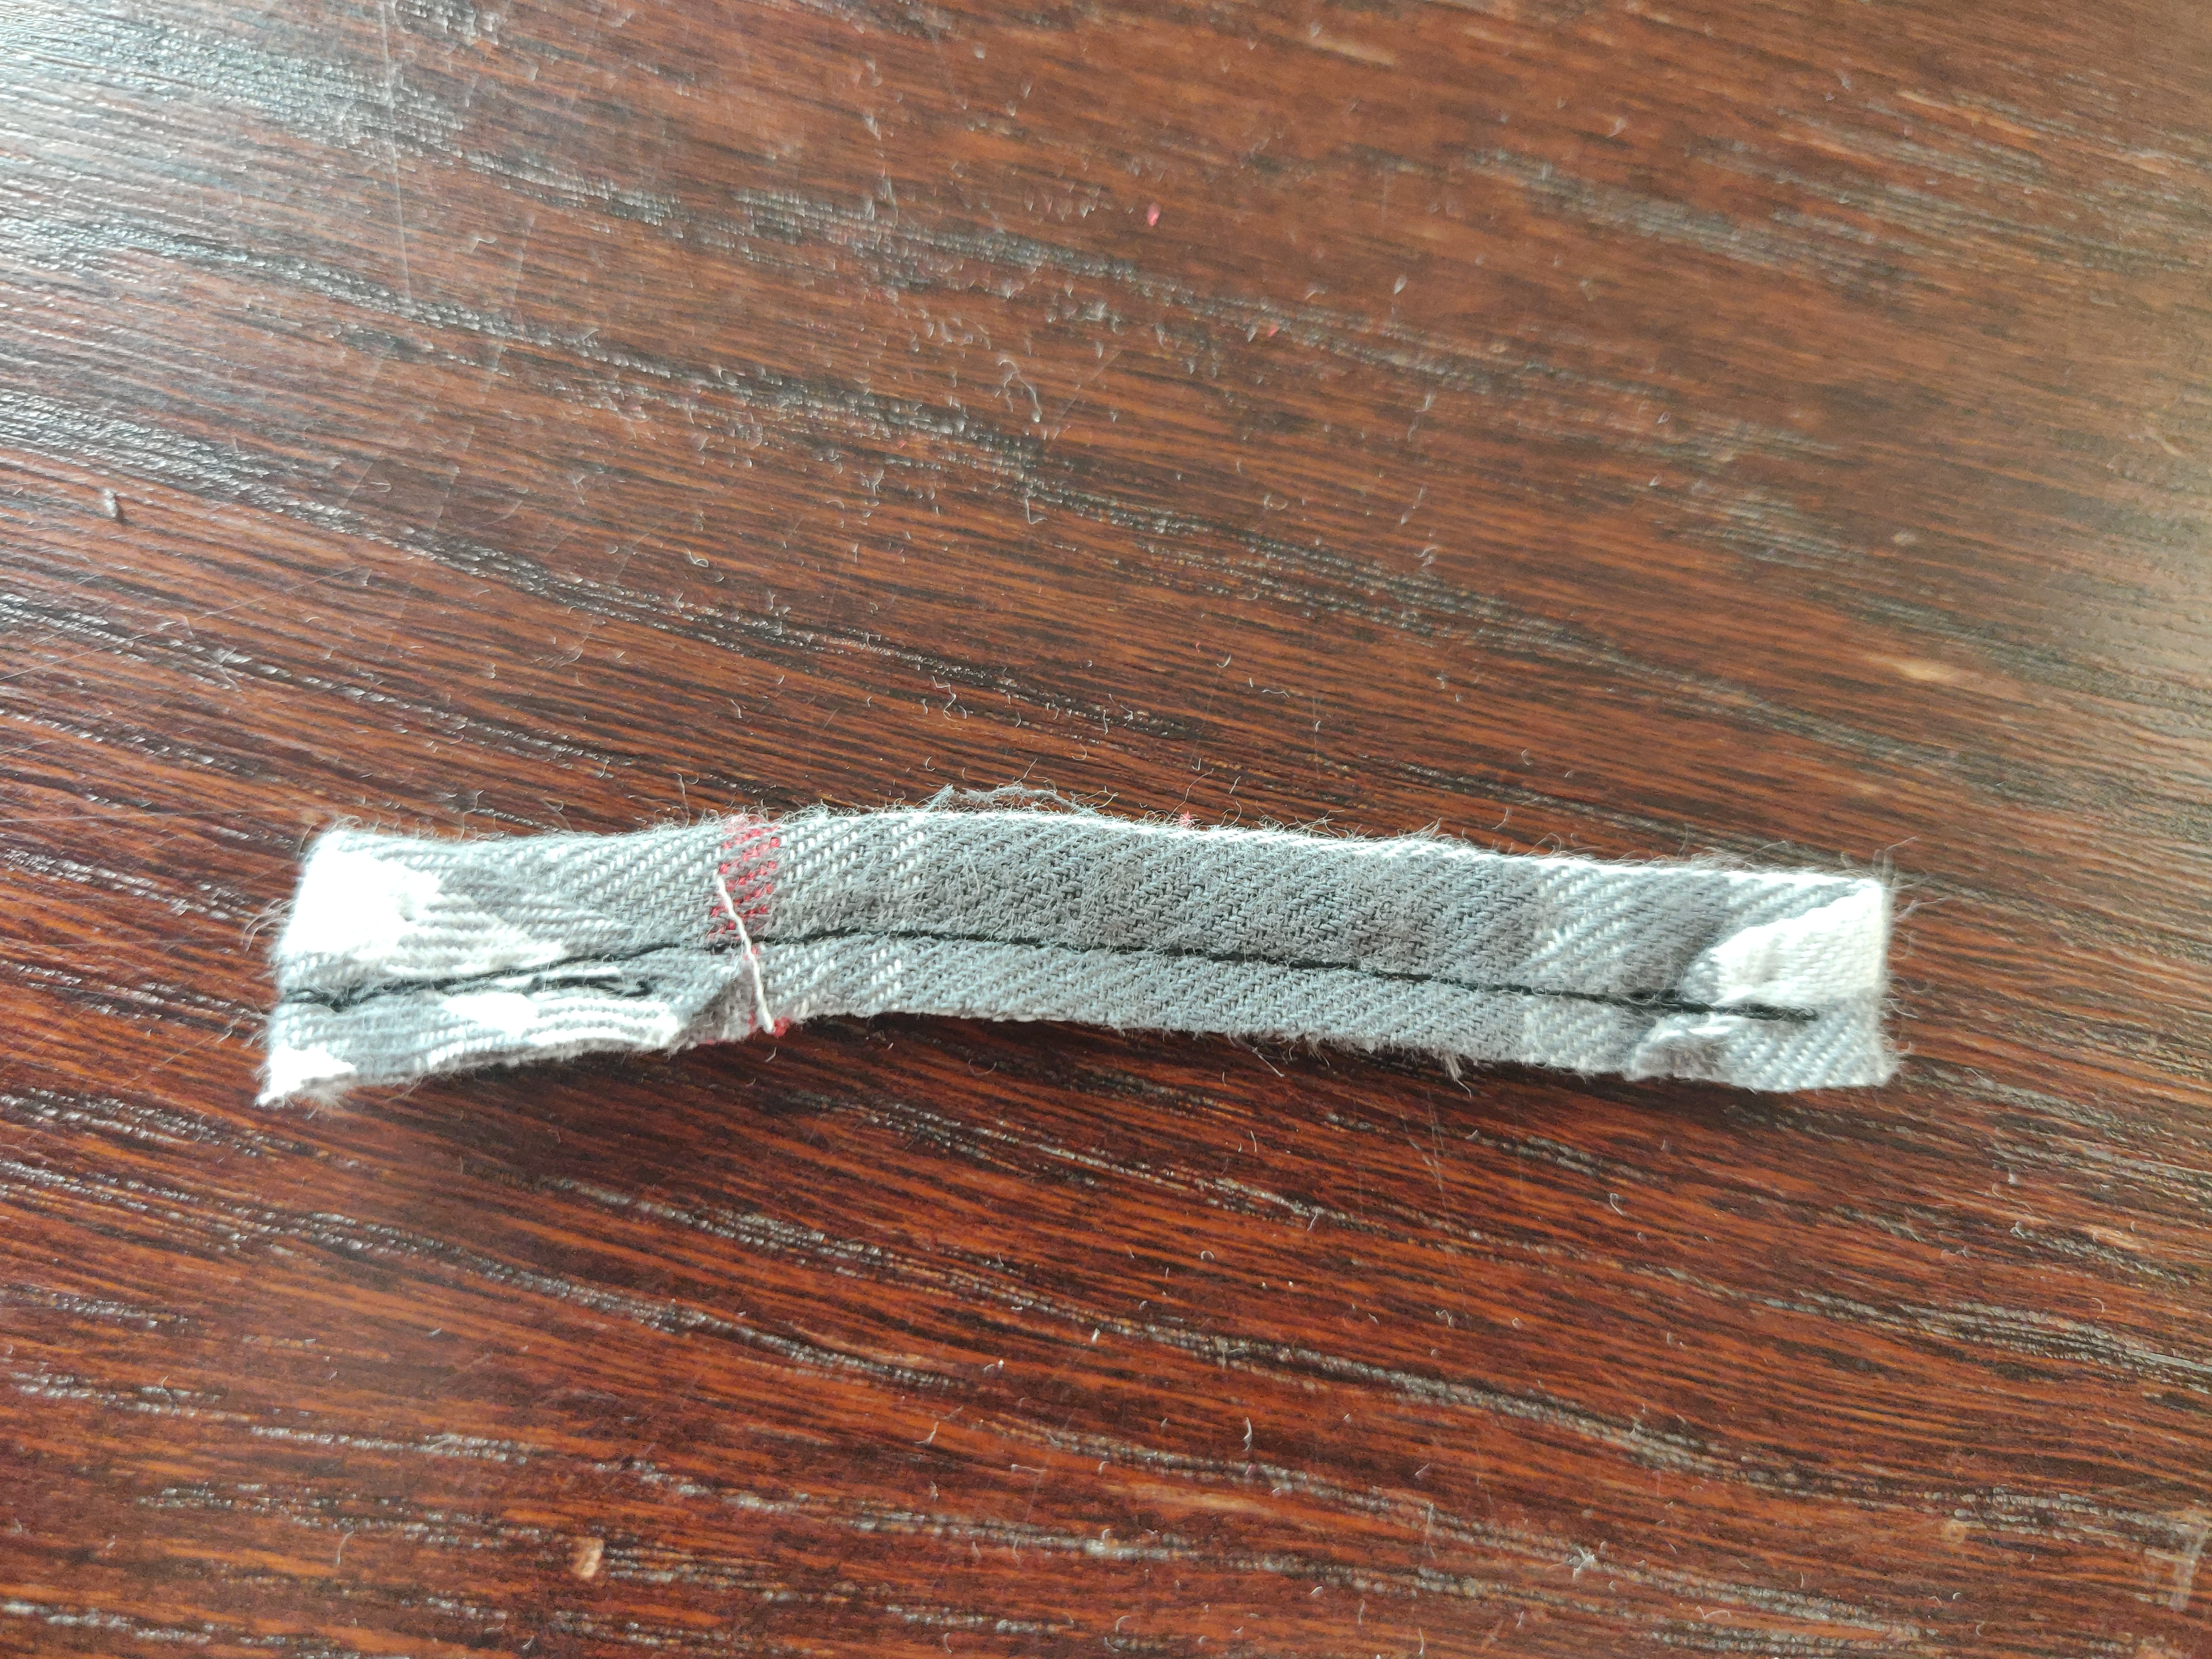
\includegraphics[width = \linewidth]{Pictures/02_MetalStrip/MetalStrip_04.jpg}
        \caption{Vernäht und Zugeschnitten}
        \label{MetaStrip4}
    \end{subfigure}
    \caption{Drahteinsatz in Stoff einnähen}
    \label{MetaStrip}
\end{figure}

\end{document}
